\chapter{अभिक्रिया दरों के सिद्धांत}\label{ch:b3:rate-theories}

2017 में एक ऐसी औषधि को स्वीकृति मिली जिसका एक पुरानी औषधि से एकमात्र अंतर यह है
कि उसके दो मेथॉक्सी समूहों के छह हाइड्रोजन परमाणु ड्यूटेरियम परमाणु हैं।
यकृत औषधि को ठीक उन्हीं C--H आबंधों को काटकर विघटित करता है, और C--D आबंध
कई गुना धीरे कटता है: भारी अणु रक्त में अधिक देर तक रहता है, और
छोटी, कम बार की खुराकों में लिया जाता है। आरेनियस
नियम में कुछ भी यह नहीं समझाता कि नाभिक में एक न्यूट्रॉन किसी अभिक्रिया को धीमा क्यों करे। यह
अध्याय दर स्थिरांकों को आण्विक गुणधर्मों से व्युत्पन्न करता है: पहले
संघट्टों से, फिर \omterm{def:b3:computational-chemistry:pes}{स्थितिज ऊर्जा पृष्ठ} की आकृति और
\omterm{def:b3:rate-theories:tst}{संक्रमण-अवस्था सिद्धांत} के विभाजन फलनों से, जो ऐसे समस्थानिक प्रभावों के आकार की
भविष्यवाणी करता है; यह विलयन में अभिक्रियाओं पर समाप्त होता है, जहाँ विलायक
एक गति-सीमा निर्धारित करता है।

\begin{recall}
प्रथम वर्ष के खंड ने दर स्थिरांक, आरेनियस नियम $k =
A\eu^{-E_a/RT}$, उसकी सक्रियण ऊर्जा और पूर्व-घातांकी गुणक, मूल
चरण, संक्रमण अवस्था, अभिक्रिया निर्देशांक के अनुदिश ऊर्जा प्रोफ़ाइल
और हैमंड अभिगृहीत परिभाषित किए। द्वितीय वर्ष के खंड ने आयनिक सामर्थ्य और सक्रियता
गुणांक परिभाषित किए, डिबाई--ह्युकेल सीमांत नियम $\log\gamma_i = -Az_i^2\sqrt I$ के साथ ($A \approx
0.51$, \qty{25}{\celsius} पर जल में), और न्यूनतम-वर्ग रेखाएँ समंजित कीं।
\Cref{ch:b3:computational-chemistry} ने \omterm{def:b3:computational-chemistry:pes}{स्थितिज ऊर्जा पृष्ठों} का परिचय दिया;
\cref{ch:b3:partition-functions,ch:b3:statistical-thermo-applied} ने विभाजन फलनों
और \omterm{def:b3:quantum-model-systems:oscillator}{शून्य-बिंदु ऊर्जाओं} से साम्य स्थिरांक परिकलित किए। भौतिकी
से: आण्विक चालों का मैक्सवेल--बोल्ट्समान वितरण, और विसरण का फ़िक
नियम।
\end{recall}

\begin{omfigure}
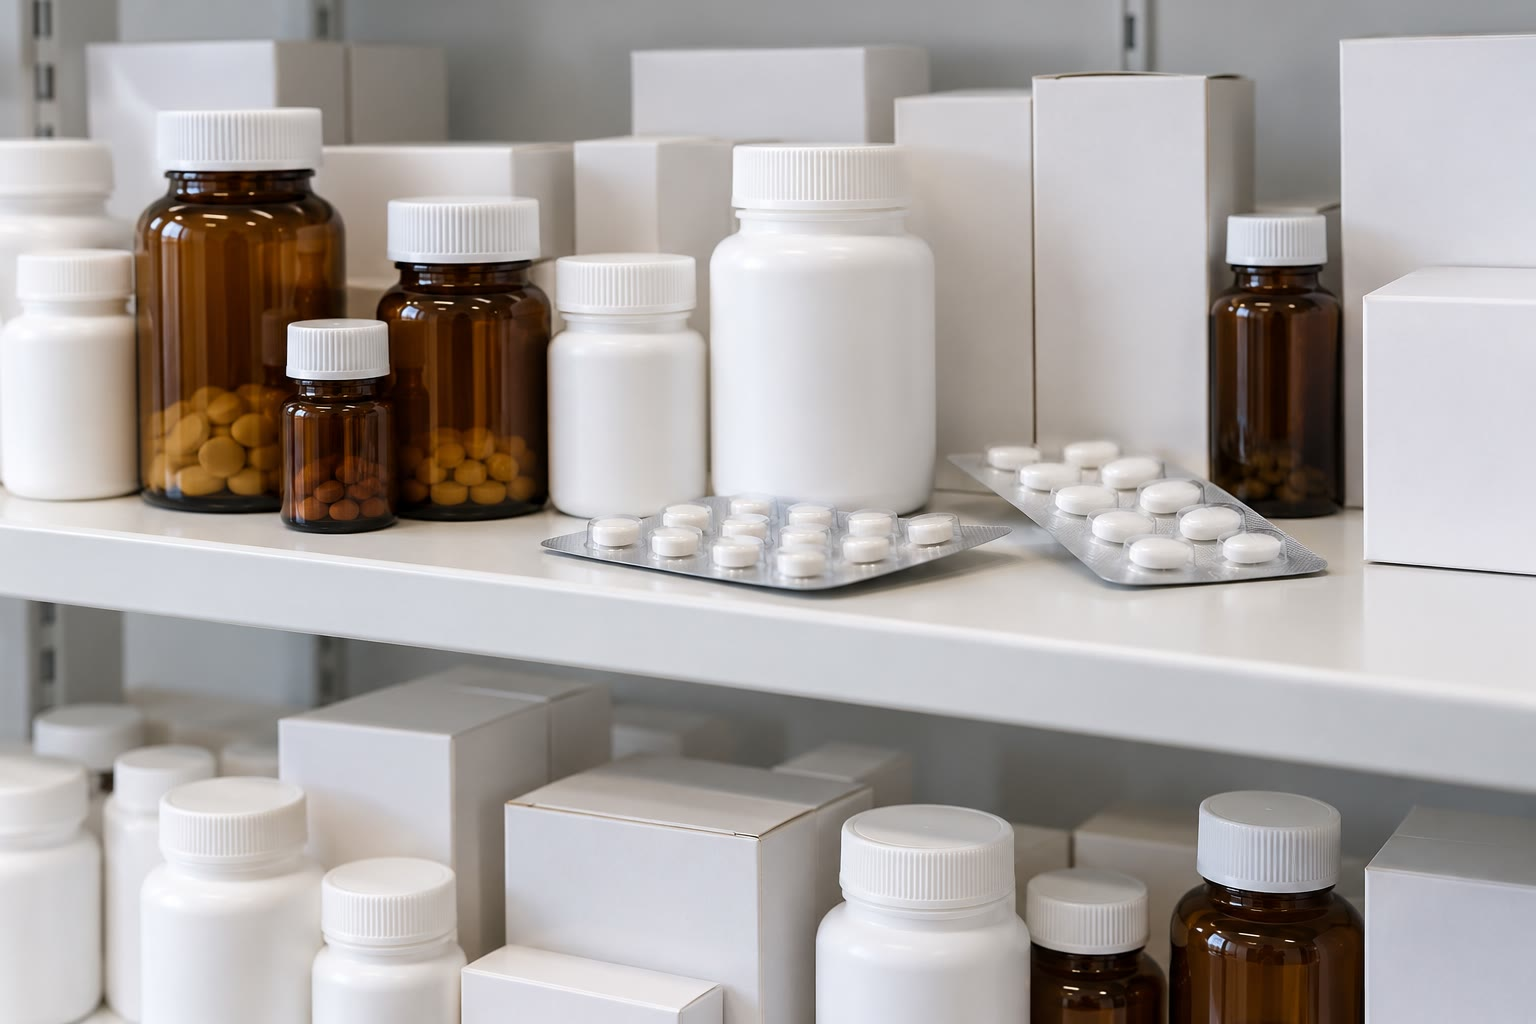
\includegraphics[width=0.6\linewidth]{images/book4/ai/b3-12-pharmacy.jpg}

{\small एक फ़ार्मेसी की शेल्फ़ पर औषधियाँ। उन आबंधों पर हाइड्रोजन के स्थान पर ड्यूटेरियम
रखने से, जिन पर यकृत सबसे पहले आक्रमण करता है, औषधि के शरीर में रहने का समय बढ़ सकता है।}
\end{omfigure}

\section{संघट्ट सिद्धांत}

गैस में दो अणु केवल तभी अभिक्रिया कर सकते हैं जब वे मिलें। उन्हें व्यास $d_{\mathrm A}$ और $d_{\mathrm B}$
वाले कठोर गोलों के रूप में मॉडल कीजिए: वे तब संघट्टित होते हैं जब उनके केंद्र एक-दूसरे से $d =
\frac12(d_{\mathrm A} + d_{\mathrm B})$ के भीतर से गुज़रते हैं।

\begin{definition}[संघट्ट अनुप्रस्थ-काट, त्रिविम गुणक]\label{def:b3:rate-theories:collision}
दो अणुओं का \emph{संघट्ट अनुप्रस्थ-काट}\index{संघट्ट अनुप्रस्थ-काट}
उनके आपेक्षिक वेग के लंबवत चकती का क्षेत्रफल $\sigma = \pi d^2$ है,
जिसके भीतर से एक के केंद्र को गुज़रना चाहिए ताकि वह दूसरे से टकराए।
\emph{त्रिविम गुणक}\index{त्रिविम गुणक} $P$ किसी अभिक्रिया के मापे गए
पूर्व-घातांकी गुणक और संघट्ट सिद्धांत द्वारा अनुमानित गुणक का अनुपात है।
\end{definition}

\begin{omfigure}
\begin{tikzpicture}[font=\small, >=Stealth]
  \shade[ball color=omDef!40] (0,0) circle (0.45);
  \node at (0,0) {A};
  \draw[black!50, dashed] (-0.0,0.85) -- (5.2,0.85) (-0.0,-0.85) -- (5.2,-0.85);
  \draw[black!60] (0,0) ellipse (0.25 and 0.85);
  \draw[<->] (-0.45,0) -- (-0.45,0.85) node[midway, left] {$d$};
  \shade[ball color=omThm!40] (3.3,0.55) circle (0.4);
  \node at (3.3,0.55) {B};
  \shade[ball color=omThm!20] (4.6,1.45) circle (0.4);
  \node at (4.6,1.45) {B};
  \draw[->, thick] (0.6,0) -- (2.2,0) node[midway, below] {$v_{\mathrm{rel}}\,\Delta t$};
  \node[anchor=west, align=left, font=\scriptsize] at (5.3,0) {अनुप्रस्थ-काट\\ $\sigma = \pi d^2$\\ का बेलन};
  \node[font=\scriptsize, anchor=south] at (3.3,1.0) {टकराया};
  \node[font=\scriptsize, anchor=south] at (4.6,1.9) {चूक};
\end{tikzpicture}

{\small संघट्ट बेलन। आपेक्षिक चाल $v_{\mathrm{rel}}$ से चलता अणु A
समय $\Delta t$ में अनुप्रस्थ-काट $\sigma = \pi d^2$ का एक बेलन बुहारता है, जहाँ $d$ दोनों
त्रिज्याओं का योग है; हर B जिसका केंद्र भीतर है, टकराया जाता है।}
\end{omfigure}

\begin{theorem}[संघट्ट-सिद्धांत दर स्थिरांक]\label{thm:b3:rate-theories:collision}
यदि हर वह संघट्ट जिसकी केंद्र-रेखा के अनुदिश गतिज ऊर्जा
देहली $E_0$ (प्रति मोल) से अधिक है, अभिक्रिया तक ले जाता है, तो $\mathrm{A + B} \to$
उत्पाद का दर स्थिरांक यह है:
\[
  k = \sigma\bar v_{\mathrm{rel}}N_A\,\eu^{-E_0/RT}, \qquad \bar v_{\mathrm{rel}} = \sqrt{\frac{8kT}{\pi\mu}},\
  \mu = \frac{m_{\mathrm A}m_{\mathrm B}}{m_{\mathrm A} + m_{\mathrm B}} .
\]
\end{theorem}

\begin{proof}[आंशिक उपपत्ति]
समय $\Delta t$ में अणु A आयतन $\sigma v_{\mathrm{rel}}\Delta t$ बुहारता है और उसमें स्थित
$n_{\mathrm B}\sigma v_{\mathrm{rel}}\Delta t$ अणुओं B से टकराता है: प्रति एकक आयतन संघट्ट दर
$\sigma\bar v_{\mathrm{rel}}n_{\mathrm A}n_{\mathrm B}$ है, जहाँ $\bar v_{\mathrm{rel}}$ माध्य आपेक्षिक चाल है जो
मैक्सवेल--बोल्ट्समान वितरण देता है (भौतिकी से स्वीकृत, \omterm{def:b3:quantum-model-systems:oscillator}{समानीत
द्रव्यमान} के साथ)। हर संघट्ट को उसकी चाल से भारित करने और उन्हें रखने पर जिनकी ऊर्जा
केंद्र-रेखा के अनुदिश देहली से अधिक है, संघट्ट दर का अंश
$\eu^{-E_0/RT}$ बचता है (संघट्ट प्राचल पर समाकलन
स्वीकृत है)। संख्या घनत्वों को मोलर सांद्रताओं में बदलने पर
$N_A$ से गुणा होता है।
\end{proof}

चूँकि $\bar v_{\mathrm{rel}} \propto \sqrt T$, सक्रियण ऊर्जा $E_a = RT^2\,\dd\ln k/\dd T$, $E_0 + \frac12RT$ है,
देहली के निकट। छोटे अणुओं के लिए पूर्व-घातांकी गुणक
$10^{11}$~\unit{L.mol^{-1}.s^{-1}} की कोटि का है। मापे गए गुणक प्रायः
कहीं छोटे होते हैं: $P \ll 1$ उन अणुओं के लिए जिन्हें किसी विशेष
अभिविन्यास में मिलना होता है, और वास्तविक अणुओं के लिए, जो कठोर गोले नहीं हैं,
अनुप्रस्थ-काट का कोई एक मान नहीं होता। संघट्ट सिद्धांत परिमाण की कोटि और
ताप-निर्भरता देता है; वह $E_0$ नहीं दे सकता, जिसके लिए \omterm{def:b3:computational-chemistry:pes}{स्थितिज
ऊर्जा पृष्ठ} चाहिए।

\section{स्थितिज ऊर्जा पृष्ठ}

अभिक्रिया $\mathrm{H_A + H_BH_C \to H_AH_B + H_C}$ सबसे सरल है। संरेख
पहुँच के लिए ऊर्जा दो दूरियों, $r_{\mathrm{AB}}$ और $r_{\mathrm{BC}}$, पर निर्भर करती है, और उसे
एक मानचित्र के रूप में खींचा जा सकता है।

\begin{definition}[पल्याण बिंदु, न्यूनतम ऊर्जा पथ]\label{def:b3:rate-theories:saddle}
\omterm{def:b3:computational-chemistry:pes}{स्थितिज ऊर्जा पृष्ठ} का \emph{पल्याण बिंदु}\index{पल्याण बिंदु} वह बिंदु है
जहाँ प्रवणता लुप्त होती है, ऊर्जा एक दिशा के अनुदिश अधिकतम और अन्य सभी के अनुदिश
न्यूनतम होती है। \emph{न्यूनतम ऊर्जा पथ}\index{न्यूनतम ऊर्जा पथ}
पल्याण बिंदु से अभिकारक और उत्पाद घाटियों तक तीव्रतम अवरोहण का पथ है;
उसके अनुदिश मापी गई उसकी लंबाई अभिक्रिया निर्देशांक है,
और पल्याण बिंदु संक्रमण अवस्था है।
\end{definition}

\begin{omfigure}
\begin{tikzpicture}
\begin{axis}[ompes, width=0.62\linewidth, xmin=0.4, xmax=3.0, ymin=0.4, ymax=3.0,
  xlabel={$r_{\mathrm{AB}}$ / \AA}, ylabel={$r_{\mathrm{BC}}$ / \AA},
  colorbar, colorbar style={ylabel={$E$ / eV}, ylabel style={font=\small},
  yticklabel style={font=\small}}, point meta min=-4.7, point meta max=-0.8]
\addplot3[contour prepared={labels=false}, thick] table {figdata/out/bachelor-3-pes-collinear-contours.dat};
\addplot3[ompath] table[x=x, y=y, z expr=0] {figdata/out/bachelor-3-pes-collinear-mep.dat};
\node[omsaddle] at (axis cs:0.918,0.918,0) {};
\node[font=\small, anchor=south west] at (axis cs:0.95,0.95,0) {पल्याण};
\node[font=\small, anchor=west, fill=white, fill opacity=0.85, text opacity=1, inner sep=1.5pt] at (axis cs:2.05,1.0,0) {$\mathrm{H_A + H_BH_C}$};
\node[font=\small, anchor=west, fill=white, fill opacity=0.85, text opacity=1, inner sep=1.5pt] at (axis cs:0.95,2.55,0) {$\mathrm{H_AH_B + H_C}$};
\node[font=\small, anchor=north east] at (axis cs:2.95,2.95,0) {$\ce{H + H + H}$};
\end{axis}
\end{tikzpicture}

{\small संरेख $\ce{H + H2}$ के लिए एक मॉडल \omterm{def:b3:computational-chemistry:pes}{स्थितिज ऊर्जा पृष्ठ} (\ce{H2} के मोर्स वक्र से बना LEPS रूप,
मॉडल स्थिरांक के रूप में चुने गए सातो प्राचल 0.17 के साथ)।
\qty{-4.65}{eV} से \qty{-0.8}{eV} तक समोच्च, तीन अलग परमाणुओं के लिए ऊर्जा शून्य;
घाटियाँ \qty{-4.75}{eV} पर हैं, जो \ce{H2} कूप की गहराई है। खंडित: \omterm{def:b3:rate-theories:saddle}{न्यूनतम
ऊर्जा पथ}, जो सममित पल्याण को $r_{\mathrm{AB}} = r_{\mathrm{BC}} = \qty{0.92}{\angstrom}$ पर पार करता है,
इस मॉडल में घाटियों से \qty{0.27}{eV} ऊपर।}
\end{omfigure}

पथ अभिकारक घाटी से ऊपर चढ़ता है, जहाँ A के निकट आने के दौरान $r_{\mathrm{BC}}$, \ce{H2}
आबंध लंबाई के निकट रहता है, पल्याण को पार करता है, और
उत्पाद घाटी में उतरता है। पल्याण पर दोनों आबंध \qty{0.92}{\angstrom} तक खिंचे हैं: पुराना
आबंध आधा टूटा है और नया आधा बना, और इस समझौते की ऊर्जा
कीमत ही अवरोध है। सममित अभिक्रिया के लिए पल्याण
विकर्ण पर होता है; ऊष्माक्षेपी अभिक्रिया के लिए वह अभिकारक घाटी की ओर खिसकता है (एक
आरंभिक अवरोध, अभिकारक-सदृश संक्रमण अवस्था, जैसा हैमंड अभिगृहीत
कहता है), ऊष्माशोषी के लिए उत्पाद घाटी की ओर (एक पश्च अवरोध)।
स्थिति तय करती है कि कौन-सी ऊर्जा सहायक है: स्थानांतरणीय ऊर्जा, जो
प्रवेश घाटी के अनुदिश निर्देशित है, अणुओं को आरंभिक अवरोध के पार ले जाती है; पश्च
अवरोध, जो एक मोड़ के पार है, टूटते आबंध में कंपनिक ऊर्जा होने पर अधिक आसानी से
पार होता है। ये पोलान्यी के नियम हैं, जिनकी पुष्टि आण्विक-पुंज
प्रयोगों ने की।

\section{संक्रमण-अवस्था सिद्धांत}

\begin{definition}[सक्रियित संकुल]\label{def:b3:rate-theories:activated-complex}
किसी मूल चरण का \emph{सक्रियित संकुल}\index{सक्रियित संकुल}
अभिक्रियारत निकाय के उन विन्यासों का समुच्चय है जो \omterm{def:b3:rate-theories:saddle}{पल्याण बिंदु} के चारों ओर,
\omterm{def:b3:rate-theories:saddle}{न्यूनतम ऊर्जा पथ} के लंबवत, एक पतली परत में हैं; उसे एक
स्पीशीज़ $\ce{AB^{\ddagger}}$ माना जाता है, जिसका अपना विभाजन फलन है।
\end{definition}

\begin{definition}[संक्रमण-अवस्था सिद्धांत, पारगमन गुणांक]\label{def:b3:rate-theories:tst}
\emph{संक्रमण-अवस्था सिद्धांत}\index{संक्रमण-अवस्था सिद्धांत} यह मानता है कि
\omterm{def:b3:rate-theories:activated-complex}{सक्रियित संकुल} अभिकारकों के साथ साम्य में हैं, कि पल्याण क्षेत्र को उत्पादों की ओर पार करने वाला
हर संकुल उन्हें बनाने तक जाता है, और कि
अभिक्रिया निर्देशांक के अनुदिश गति एक मुक्त स्थानांतरण है।
\emph{पारगमन गुणांक}\index{पारगमन गुणांक} $\kappa \le 1$ उन संकुलों के लिए संशोधन करता है
जो वापस अभिकारकों की ओर पुनः पार कर जाते हैं।
\end{definition}

\begin{theorem}[आयरिंग समीकरण]\label{thm:b3:rate-theories:eyring}
मूल चरण $\mathrm{A + B} \to \mathrm{AB}^{\ddagger} \to$ उत्पाद के लिए,
\[
  k = \kappa\frac{k_BT}{h}\overline{K}{}^{\ddagger}, \qquad
  \overline{K}{}^{\ddagger} = \frac{\bar q^{\ddagger}/N_A}{(q_{\mathrm A}/N_A)(q_{\mathrm B}/N_A)}\,\eu^{-\Delta E_0^{\ddagger}/RT},
\]
जहाँ $\bar q^{\ddagger}$ \omterm{def:b3:rate-theories:activated-complex}{सक्रियित संकुल} का विभाजन फलन है, जिसमें से
अभिक्रिया-निर्देशांक गति हटा दी गई है, $q$ प्रति एकक आयतन मोलर विभाजन फलन हैं,
और $\Delta E_0^{\ddagger}$ संकुल के शून्य-बिंदु स्तर की अभिकारकों के शून्य-बिंदु स्तर से
ऊँचाई है। ऊष्मागतिक रूप में, $c^\circ = \qty{1}{mol/L}$ और
आण्विकता $m$ के साथ,
\[
  k = \kappa\frac{k_BT}{h}(c^\circ)^{1-m}\,\eu^{\Delta^{\ddagger}S^\circ/R}\,\eu^{-\Delta^{\ddagger}H^\circ/RT}.
\]
यह कथन \emph{आयरिंग समीकरण}\index{आयरिंग समीकरण} है; $k_B$
बोल्ट्समान स्थिरांक है, जिसे $k$ से भ्रम से बचने के लिए ऐसे लिखा गया है।
\end{theorem}

\begin{proof}
अर्ध-साम्य: $[\ce{AB^{\ddagger}}] = K^{\ddagger}[\mathrm A][\mathrm B]$, जहाँ $K^{\ddagger}$ विभाजन फलनों से है
(\cref{thm:b3:statistical-thermo-applied:k-from-q}, सांद्रताओं में लिखा गया)।
संकुल के कंपनों में से एक अभिक्रिया
निर्देशांक के अनुदिश गति है: आवृत्ति $\nu \ll k_BT/h$ का एक बहुत ढीला कंपन, जिसका विभाजन
फलन $k_BT/h\nu$ है (\cref{prop:b3:partition-functions:q-vib} की
उच्च-ताप सीमा); अतः $q^{\ddagger} = \bar q^{\ddagger}k_BT/h\nu$।
संकुल इस गति की आवृत्ति $\nu$ पर उत्पादों की ओर पार करते हैं, अतः
दर $\nu[\ce{AB^{\ddagger}}] = \nu\frac{k_BT}{h\nu}\overline{K}{}^{\ddagger}[\mathrm A][\mathrm B]$ है: अज्ञात $\nu$ निरस्त हो जाता है।
$\overline{K}{}^{\ddagger} = (c^\circ)^{1-m}\eu^{-\Delta^{\ddagger}G^\circ/RT}$ और $\Delta^{\ddagger}G^\circ = \Delta^{\ddagger}H^\circ - T\Delta^{\ddagger}S^\circ$ लिखने पर
दूसरा रूप मिलता है, पुनः-पारण के लिए $\kappa$ जोड़कर।
\end{proof}

गुणक $k_BT/h$, \qty{298}{K} पर \qty{6.2e12}{s^{-1}} है: बिना अवरोध और बिना एन्ट्रॉपी-हानि
वाले एकाण्विक चरण की दर। अभिक्रिया की हर विशिष्टता
सक्रियण की राशियों में निहित है।

\begin{definition}[सक्रियण की गिब्स ऊर्जा, एन्थैल्पी और एन्ट्रॉपी]\label{def:b3:rate-theories:activation}
किसी मूल चरण की \emph{सक्रियण की गिब्स ऊर्जा}\index{सक्रियण की गिब्स ऊर्जा}
$\Delta^{\ddagger}G^\circ$, \emph{सक्रियण की एन्थैल्पी}\index{सक्रियण की एन्थैल्पी} $\Delta^{\ddagger}H^\circ$ और
\emph{सक्रियण की एन्ट्रॉपी}\index{सक्रियण की एन्ट्रॉपी} $\Delta^{\ddagger}S^\circ$
अभिकारकों से \omterm{def:b3:rate-theories:activated-complex}{सक्रियित संकुल} (उसकी अभिक्रिया-निर्देशांक गति के बिना) के संभवन की
मानक गिब्स ऊर्जा, एन्थैल्पी और एन्ट्रॉपी हैं, जो
\omterm{thm:b3:rate-theories:eyring}{आयरिंग समीकरण} द्वारा परिभाषित होती हैं।
\end{definition}

\begin{proposition}[सक्रियण ऊर्जा और सक्रियण की एन्थैल्पी]\label{prop:b3:rate-theories:ea-dh}
विलयन में अभिक्रिया के लिए $E_a = \Delta^{\ddagger}H^\circ + RT$; द्विआण्विक गैस अभिक्रिया के लिए
$E_a = \Delta^{\ddagger}H^\circ + 2RT$।
\end{proposition}

\begin{proof}
$E_a = RT^2\,\dd\ln k/\dd T$, और $\ln k = \ln T + \Delta^{\ddagger}S^\circ/R - \Delta^{\ddagger}H^\circ/RT + $ अचर: $E_a =
RT + \Delta^{\ddagger}H^\circ$, जब सक्रियण प्राचल $T$ के साथ नहीं बदलते। विलयन में
यही परिणाम है। गैस प्रावस्था में सांद्रताओं में लिखे $K^{\ddagger}$ के लिए वांट हॉफ़ संबंध
में आंतरिक ऊर्जा आती है, $\Delta^{\ddagger}U^\circ = \Delta^{\ddagger}H^\circ - \Delta n^{\ddagger}RT$,
जहाँ $\Delta n^{\ddagger} = 1 - m$: $m = 2$ के लिए $E_a = \Delta^{\ddagger}H^\circ + 2RT$।
\end{proof}

\omterm{def:b3:rate-theories:activation}{सक्रियण की एन्ट्रॉपी} संक्रमण अवस्था की संरचना पढ़ती है। दो
अणु जो मिलकर एक संकुल बनाते हैं, स्थानांतरणीय और घूर्णी
स्वातंत्र्य खोते हैं: $\Delta^{\ddagger}S^\circ$ प्रबल रूप से ऋणात्मक है, $-50$ से $-150$ \unit{J.K^{-1}.mol^{-1}},
साहचर्यी चरणों और चक्रीय संक्रमण अवस्थाओं के लिए। जो अणु वियोजन की राह में कोई आबंध
ढीला करता है, वह स्वातंत्र्य प्राप्त करता है: $\Delta^{\ddagger}S^\circ > 0$।

\begin{proposition}[समंजित रेखा की मानक त्रुटियाँ]\label{prop:b3:rate-theories:slope-uncertainty}
न्यूनतम-वर्ग रेखा $y = a + bx$ के लिए, जो $n$ बिंदुओं से होकर जाती है, जिनके $y$ में
समान प्रसरण की स्वतंत्र त्रुटियाँ हैं, जिसका आकलन $s^2 = \sum_i(y_i - a - bx_i)^2/(n - 2)$ है,
ढलान और अंतःखंड की मानक त्रुटियाँ ये हैं:
\[
  s_b = \frac{s}{\sqrt{\sum_i(x_i - \bar x)^2}}, \qquad
  s_a = s\sqrt{\frac1n + \frac{\bar x^2}{\sum_i(x_i - \bar x)^2}} .
\]
\end{proposition}

\begin{proof}
$b = \sum_i(x_i - \bar x)y_i/S_{xx}$, जहाँ $S_{xx} = \sum_i(x_i - \bar x)^2$, स्वतंत्र $y_i$ का, जिनका
प्रसरण $\sigma^2$ है, एक रैखिक संयोजन है: उसका प्रसरण $\sigma^2\sum_i(x_i - \bar x)^2/S_{xx}^2 = \sigma^2/S_{xx}$ है।
इसी प्रकार $a = \bar y - b\bar x$, और $\bar y$ तथा $b$ असहसंबद्ध हैं (उनका सहप्रसरण
$\sigma^2\sum_i(x_i - \bar x)/(nS_{xx}) = 0$ है), अतः $\operatorname{var}a = \sigma^2/n + \bar x^2\sigma^2/S_{xx}$। $\sigma^2$ के स्थान पर
उसका आकलन $s^2$ रखने पर (भाजक $n - 2$ दो समंजित
प्राचलों का ध्यान रखता है, स्वीकृत) परिणाम मिलता है।
\end{proof}

\begin{method}[अनिश्चितताओं सहित आयरिंग आलेख]\label{met:b3:rate-theories:eyring-plot}
\begin{enumerate}
  \item 30 से \qty{40}{K} में फैले पाँच या अधिक तापों पर $k$ मापिए।
  \item $y = \ln(k/T)$ को $x = 1/T$ के विरुद्ध आलेखित कीजिए और न्यूनतम-वर्ग रेखा $y = a + bx$ समंजित कीजिए।
  \item $\Delta^{\ddagger}H^\circ = -Rb$ और $\Delta^{\ddagger}S^\circ = R[a - \ln(k_B/h)]$ ($\ln(k_B/h) = 23.760$, जहाँ $k$,
        \unit{s^{-1}} में है)।
  \item उनकी मानक त्रुटियाँ $Rs_b$ और $Rs_a$ हैं; 95\,\% विश्वास्यता अंतराल
        उन्हें स्टूडेंट $t$ से गुणा करता है, $n - 2$ स्वातंत्र्य कोटियों के लिए (पाँच बिंदुओं के लिए
        3.18)।
  \item अंतःखंड मापे गए परास से बहुत बाहर, $1/T = 0$ पर, स्थित है: $\Delta^{\ddagger}S^\circ$
        सदा $\Delta^{\ddagger}H^\circ$ से कहीं कम परिशुद्ध होता है, और दोनों त्रुटियाँ
        सहसंबद्ध होती हैं।
\end{enumerate}
\end{method}

\begin{omfigure}
\begin{tikzpicture}
\begin{axis}[width=0.74\linewidth, height=6.2cm, xmin=3.12, xmax=3.62, ymin=-12.8, ymax=-6.4,
  axis lines=left, xlabel={$1000\,\mathrm K/T$}, ylabel={$\ln\bigl(k/(\mathrm s^{-1}\,\mathrm K^{-1})\bigr)$},
  tick label style={font=\small}, label style={font=\small},
  legend style={font=\scriptsize, draw=none, fill=white, fill opacity=0.85, text opacity=1,
  at={(0.98,0.98)}, anchor=north east}, legend cell align=left]
\addplot[omDef, thick] table[x=invT, y=fit] {figdata/out/bachelor-3-eyring-band-H.dat};
\addplot[omThm, thick] table[x=invT, y=fit] {figdata/out/bachelor-3-eyring-band-D.dat};
\addplot[omDef, thin, dashed, forget plot] table[x=invT, y=lo] {figdata/out/bachelor-3-eyring-band-H.dat};
\addplot[omDef, thin, dashed, forget plot] table[x=invT, y=hi] {figdata/out/bachelor-3-eyring-band-H.dat};
\addplot[omThm, thin, dashed, forget plot] table[x=invT, y=lo] {figdata/out/bachelor-3-eyring-band-D.dat};
\addplot[omThm, thin, dashed, forget plot] table[x=invT, y=hi] {figdata/out/bachelor-3-eyring-band-D.dat};
\addplot[only marks, mark=*, mark size=1.8pt, omDef, forget plot] table[x=invT, y=lnkT_H] {figdata/out/bachelor-3-eyring-points.dat};
\addplot[only marks, mark=square*, mark size=1.7pt, omThm, forget plot] table[x=invT, y=lnkT_D] {figdata/out/bachelor-3-eyring-points.dat};
\legend{\ce{OCH3} औषधि, \ce{OCD3} औषधि}
\end{axis}
\end{tikzpicture}

{\small सप्ताहांत समस्या के दर स्थिरांकों (समस्या के
आँकड़े) के आयरिंग आलेख, औषधि और उसके ड्यूटेरीकृत अनुरूप के लिए, न्यूनतम-वर्ग रेखाओं
और उनके 95\,\% विश्वास्यता पट्टों (खंडित, रेखाओं से मुश्किल से चौड़े: बिंदु
लगभग 1\,\% बिखरे हैं) के साथ। रेखाएँ अपनी
अनिश्चितता के भीतर समांतर हैं: \omterm{def:b3:rate-theories:activation}{सक्रियण की एन्ट्रॉपी} समान, \omterm{def:b3:rate-theories:activation}{सक्रियण की एन्थैल्पियाँ}
लगभग \qty{5}{kJ/mol} भिन्न।}
\end{omfigure}

\section{गतिक समस्थानिक प्रभाव}

\begin{definition}[गतिक समस्थानिक प्रभाव]\label{def:b3:rate-theories:kie}
किसी चरण का \emph{गतिक समस्थानिक प्रभाव}\index{गतिक समस्थानिक प्रभाव}
दो \omterm{def:b3:rovibrational-spectroscopy:rotational-constant}{समस्थानिकरूपियों} के लिए उसके दर स्थिरांकों का अनुपात $k_{\mathrm{light}}/k_{\mathrm{heavy}}$ है, प्रायः
$k_{\mathrm H}/k_{\mathrm D}$। यह \emph{प्राथमिक गतिक समस्थानिक प्रभाव}\index{प्राथमिक गतिक समस्थानिक प्रभाव}
है जब प्रतिस्थापित परमाणु से आबंध उस चरण में बनता या टूटता है,
\emph{द्वितीयक गतिक समस्थानिक प्रभाव}\index{द्वितीयक गतिक समस्थानिक प्रभाव}
जब ऐसा नहीं होता।
\end{definition}

\begin{proposition}[अधिकतम प्राथमिक गतिक समस्थानिक प्रभाव]\label{prop:b3:rate-theories:primary-kie}
यदि X--H आबंध का तनन कंपन अभिक्रिया निर्देशांक बन जाता है,
जिससे उसकी \omterm{def:b3:quantum-model-systems:oscillator}{शून्य-बिंदु ऊर्जा} संक्रमण अवस्था में खो जाती है जबकि बाकी सभी
योगदान H और D के लिए समान रहते हैं,
\[
  \frac{k_{\mathrm H}}{k_{\mathrm D}} = \exp\Bigl[\frac{hc(\tilde\nu_{\mathrm{XH}} - \tilde\nu_{\mathrm{XD}})}{2k_BT}\Bigr],
  \qquad \frac{\tilde\nu_{\mathrm{XH}}}{\tilde\nu_{\mathrm{XD}}} = \sqrt{\frac{\mu_{\mathrm{XD}}}{\mu_{\mathrm{XH}}}} .
\]
\end{proposition}

\begin{proof}
\omterm{def:b3:computational-chemistry:pes}{स्थितिज ऊर्जा पृष्ठ} दोनों \omterm{def:b3:rovibrational-spectroscopy:rotational-constant}{समस्थानिकरूपियों} के लिए एक ही है (इलेक्ट्रॉन
न्यूट्रॉन को नहीं देखते)। अभिकारक में X--H तनन
$\frac12hc\tilde\nu_{\mathrm{XH}}$ \omterm{def:b3:quantum-model-systems:oscillator}{शून्य-बिंदु ऊर्जा} रखता है; संक्रमण अवस्था में यह विधा
अभिक्रिया निर्देशांक बन चुकी है और कोई ऊर्जा नहीं रखती। शून्य-बिंदु
स्तरों के बीच मापा गया अवरोध इसलिए H के लिए $\frac12hc\tilde\nu_{\mathrm{XH}}$ से और D के लिए $\frac12hc\tilde\nu_{\mathrm{XD}}$ से कम है: $\Delta E_0^{\ddagger}(\mathrm D) -
\Delta E_0^{\ddagger}(\mathrm H) = \frac12hc(\tilde\nu_{\mathrm{XH}} - \tilde\nu_{\mathrm{XD}})$, और जब
अन्य गुणक निरस्त होते हैं तो \omterm{thm:b3:rate-theories:eyring}{आयरिंग समीकरण} अनुपात देता है। किसी तनन की तरंग-संख्या
$1/\sqrt\mu$ के समानुपाती है (\cref{ch:b3:rovibrational-spectroscopy})।
\end{proof}

\begin{omfigure}
\begin{tikzpicture}[font=\small, >=Stealth, x=1cm, y=1cm]
  \draw[->] (-1.4,0) -- (-1.4,4.7) node[anchor=south] {$E$};
  \draw[->] (-1.4,0) -- (10.6,0) node[anchor=north east] {अभिक्रिया निर्देशांक};
  \draw[very thick, black!70] plot[smooth, tension=0.6] coordinates {(1.6,3.4) (2.1,1.6) (2.7,0.8)
    (3.3,0.6) (3.9,0.8) (4.7,2.0) (5.5,3.6) (6.2,4.0) (6.9,3.6) (7.7,2.2) (8.5,1.2) (9.2,1.0)
    (9.9,1.2) (10.4,1.7)};
  \draw[black!50, dashed] (2.8,0.6) -- (3.8,0.6);
  \draw[omDef, thick] (2.42,1.35) -- (4.2,1.35);
  \draw[omThm, thick] (2.5,1.05) -- (4.05,1.05);
  \node[omDef, font=\scriptsize, anchor=south] at (3.3,1.37) {C--H};
  \node[omThm, font=\scriptsize, anchor=north] at (3.3,1.03) {C--D};
  \draw[black, thick] (5.7,4.0) -- (6.7,4.0);
  \draw[black!40, densely dotted] (0.0,4.0) -- (5.7,4.0);
  \draw[black!40, densely dotted] (0.7,1.35) -- (2.42,1.35) (0.0,1.05) -- (2.5,1.05);
  \draw[<->, omThm] (0.0,1.05) -- (0.0,4.0) node[pos=0.5, left, font=\scriptsize] {$E_0(\mathrm D)$};
  \draw[<->, omDef] (0.7,1.35) -- (0.7,4.0) node[pos=0.5, right, font=\scriptsize] {$E_0(\mathrm H)$};
  \node[anchor=south, align=center, font=\scriptsize] at (6.2,4.05) {संक्रमण अवस्था: तनन\\ अभिक्रिया निर्देशांक बन चुका है};
\end{tikzpicture}

{\small \omterm{def:b3:rate-theories:kie}{प्राथमिक गतिक समस्थानिक प्रभाव} का मूल। अभिकारक में C--H
तनन C--D तनन से अधिक \omterm{def:b3:quantum-model-systems:oscillator}{शून्य-बिंदु ऊर्जा} रखता है (कूप की तली के ऊपर के स्तर,
खंडित); संक्रमण अवस्था में यह कंपन
अभिक्रिया निर्देशांक बन चुका है, और दोनों \omterm{def:b3:rovibrational-spectroscopy:rotational-constant}{समस्थानिकरूपी} एक ही शिखर तक पहुँचते हैं।
D के लिए अवरोध \omterm{def:b3:quantum-model-systems:oscillator}{शून्य-बिंदु ऊर्जाओं} के अंतर जितना बड़ा है।}
\end{omfigure}

\begin{omfigure}
\begin{tikzpicture}
\begin{axis}[width=0.7\linewidth, height=5.6cm, xmin=200, xmax=800, ymin=1, ymax=50,
  ymode=log, axis lines=left, xlabel={$T$ / K}, ylabel={$k_{\mathrm H}/k_{\mathrm D}$ (अधिकतम)},
  tick label style={font=\small}, label style={font=\small}, log ticks with fixed point,
  ytick={1,2,5,10,20,50}, legend style={font=\scriptsize, draw=none, at={(0.98,0.98)},
  anchor=north east}, legend cell align=left]
\addplot[omThm, thick] table[x=T, y=OH] {figdata/out/bachelor-3-kie.dat};
\addplot[black!60, thick] table[x=T, y=NH] {figdata/out/bachelor-3-kie.dat};
\addplot[omDef, thick] table[x=T, y=CH] {figdata/out/bachelor-3-kie.dat};
\legend{O--H (\qty{3657}{cm^{-1}}), N--H (\qty{3337}{cm^{-1}}), C--H (\qty{2917}{cm^{-1}})}
\end{axis}
\end{tikzpicture}

{\small ताप के विरुद्ध अधिकतम \omterm{def:b3:rate-theories:kie}{प्राथमिक गतिक समस्थानिक प्रभाव}, किसी
C--H, N--H या O--H तनन की हानि के लिए (\ce{CH4}, \ce{NH3} और \ce{H2O} के \omterm{def:b3:rovibrational-spectroscopy:anharmonic}{मूल संक्रमण};
ड्यूटेरियम तरंग-संख्याएँ \omterm{def:b3:quantum-model-systems:oscillator}{समानीत द्रव्यमानों} से)। \qty{298}{K} पर C--H के लिए यह 6.5 है;
ताप बढ़ने के साथ यह 1 की ओर घटता है।}
\end{omfigure}

कक्ष ताप पर अधिकतम C--H मान, लगभग 7, एक मानदंड है। प्रेक्षित
2 से 7 के प्रभाव संकेत करते हैं कि C--H आबंध दर-निर्धारक
चरण में टूटता है; छोटे मान यह कि संक्रमण अवस्था तनन का कुछ भाग बनाए रखती है
(असममित, आरंभिक या पश्च हाइड्रोजन स्थानांतरण), या कि वह चरण
सबसे धीमा नहीं है। कक्ष ताप पर 7 से बहुत बड़े मान
\omterm{def:b3:quantum-model-systems:oscillator}{शून्य-बिंदु ऊर्जाओं} से नहीं आ सकते: वे \omterm{def:b3:quantum-model-systems:tunnelling}{सुरंगन} (\cref{ch:b3:quantum-model-systems}) प्रकट करते हैं,
जिसे दुगुने द्रव्यमान वाला कण कहीं कम करता है। द्वितीयक प्रभाव, जो
अभिक्रिया केंद्र से सटे C--H आबंधों के बंकन कंपनों के परिवर्तनों से आते हैं,
छोटे होते हैं, प्रायः प्रति ड्यूटेरियम 0.8 से 1.2; वे, उदाहरण के लिए, ऐसे
कार्बन में जो त्रिकोणीय बनता है (sp$^3$ से sp$^2$, $k_{\mathrm H}/k_{\mathrm D} > 1$) और ऐसे कार्बन में जो
चतुष्फलकीय बनता है ($< 1$), भेद करते हैं।

\begin{method}[प्रतिस्पर्धा द्वारा गतिक समस्थानिक प्रभाव का मापन]\label{met:b3:rate-theories:kie}
\begin{enumerate}
  \item अभिक्रिया दोनों \omterm{def:b3:rovibrational-spectroscopy:rotational-constant}{समस्थानिकरूपियों} के मिश्रण पर चलाइए, या ऐसे
        अणु पर जिसके एक स्थल पर H और एक तुल्य स्थल पर D हो।
  \item निम्न रूपांतरण पर रोकिए और H और D उत्पादों का अनुपात
        द्रव्यमान स्पेक्ट्रममिति या NMR से मापिए।
  \item उत्पाद अनुपात, आरंभिक अनुपात के लिए संशोधित, $k_{\mathrm H}/k_{\mathrm D}$ है; दोनों
        \omterm{def:b3:rovibrational-spectroscopy:rotational-constant}{समस्थानिकरूपी} ठीक एक जैसी परिस्थितियाँ देखते हैं, जो इस विधि को
        दो अलग दर मापनों से अधिक परिशुद्ध बनाता है।
\end{enumerate}
\end{method}

\section{विलयन में अभिक्रियाएँ}

द्रव में कोई अणु संघट्टों के बीच मुक्त रूप से नहीं उड़ता: वह
पड़ोसियों के एक पिंजरे में खड़खड़ाता है, विसरित होकर दूर जाने से पहले उनसे कई बार टकराता है।
मिलने वाले दो अभिकारक अनेक संघट्टों तक साथ रहते हैं, यही एक भेंट है।

\begin{definition}[विसरण और सक्रियण नियंत्रण, पिंजरा प्रभाव]\label{def:b3:rate-theories:diffusion}
विलयन में कोई अभिक्रिया \emph{विसरण-नियंत्रित}\index{विसरण-नियंत्रित अभिक्रिया}
है जब हर भेंट पर अभिक्रिया तीव्र हो, ताकि उसकी दर वह दर हो
जिस पर अभिकारक विसरित होकर एक साथ आते हैं; वह
\emph{सक्रियण-नियंत्रित}\index{सक्रियण-नियंत्रित अभिक्रिया} है जब भेंटों का केवल एक छोटा
अंश अभिक्रिया तक ले जाता है। \emph{पिंजरा प्रभाव}\index{पिंजरा प्रभाव}
आसपास के विलायक द्वारा अणुओं के किसी युग्म का परिरोध है,
जो उन्हें एक भेंट के दौरान बार-बार टकराने पर विवश करता है।
\end{definition}

\begin{proposition}[स्मोलुकोव्स्की सीमा]\label{prop:b3:rate-theories:smoluchowski}
ऐसे गोलों के बीच \omterm{def:b3:rate-theories:diffusion}{विसरण-नियंत्रित अभिक्रिया} का दर स्थिरांक, जो
दूरी $R^*$ पर अभिक्रिया करते हैं, $k_d = 4\pi N_A(D_{\mathrm A} + D_{\mathrm B})R^*$ है। स्टोक्स--आइंस्टाइन
संबंध $D = k_BT/6\pi\eta a$ के साथ, त्रिज्या $a$ के गोलों के लिए, श्यानता $\eta$ वाले विलायक में,
और $R^* = a_{\mathrm A} + a_{\mathrm B}$ के साथ, जहाँ $a_{\mathrm A} = a_{\mathrm B}$,
\[
  k_d = \frac{8RT}{3\eta} .
\]
\end{proposition}

\begin{proof}[आंशिक उपपत्ति]
A को मूलबिंदु पर स्थिर कीजिए; B आपेक्षिक विसरण गुणांक $D =
D_{\mathrm A} + D_{\mathrm B}$ के साथ विसरित होता है और $r = R^*$ पर नष्ट हो जाता है। स्थायी अवस्था में
हर गोले से होकर त्रिज्य अभिवाह समान है, $J = 4\pi r^2D\,\dd c/\dd r$ (फ़िक नियम,
भौतिकी से); $R^*$ से, जहाँ $c = 0$, अनंत तक, जहाँ $c = c_{\mathrm B}$, समाकलन करने पर
$J = 4\pi DR^*c_{\mathrm B}$ मिलता है, प्रति अणु A दर। स्टोक्स--आइंस्टाइन (स्वीकृत) के साथ,
$(D_{\mathrm A} + D_{\mathrm B})R^* = \frac{k_BT}{6\pi\eta}(\frac{1}{a} + \frac1a)(2a) = \frac{2k_BT}{3\pi\eta}$, और $k_d = 4\pi N_A \times
\frac{2k_BT}{3\pi\eta} = 8RT/3\eta$।
\end{proof}

\begin{example}[जल और हेक्सेन में गति-सीमाएँ]\label{ex:b3:rate-theories:speed-limit}
% ledger: visc:H2O.25C, visc:hexane.25C
\qty{298.15}{K} पर जल ($\eta = \qty{0.890}{mPa.s}$) $k_d = 8 \times 8.314 \times
298.15/(3 \times \num{0.890e-3}) = \qty{7.4e6}{m^3.mol^{-1}.s^{-1}} = \qty{7.4e9}{L.mol^{-1}.s^{-1}}$ देता है; हेक्सेन
($\eta = \qty{0.298}{mPa.s}$), \qty{2.2e10}{L.mol^{-1}.s^{-1}}। सामान्य आकार के उदासीन अणुओं के बीच कोई भी
द्विआण्विक अभिक्रिया इससे तीव्र नहीं होती; इन मानों के निकट मापे गए स्थिरांक
(उत्तेजित अवस्थाओं का शमन, मूलकों का पुनर्संयोजन)
\omterm{def:b3:rate-theories:diffusion}{विसरण-नियंत्रित} हैं। विपरीत आवेश वाले आयन आकर्षित होते हैं और अधिक तीव्र हो सकते हैं।
\end{example}

विलयन में आयन सक्रियण में एक स्थिरवैद्युत योगदान जोड़ते हैं: दो आयनों की
संक्रमण अवस्था का आवेश $z_{\mathrm A} + z_{\mathrm B}$ है, और उसका सक्रियता गुणांक
उनके गुणांकों के गुणनफल से भिन्न है।

\begin{definition}[गतिक लवण प्रभाव]\label{def:b3:rate-theories:salt}
\emph{गतिक लवण प्रभाव}\index{गतिक लवण प्रभाव} विलयन की आयनिक सामर्थ्य के साथ
आयनों के बीच किसी अभिक्रिया के दर स्थिरांक का परिवर्तन है।
\end{definition}

\begin{proposition}[ब्रॉन्स्टेड--ब्येरुम समीकरण]\label{prop:b3:rate-theories:bronsted-bjerrum}
तनु जलीय विलयन में आवेशों $z_{\mathrm A}$ और $z_{\mathrm B}$ वाले आयनों के बीच किसी चरण के लिए,
\[
  \log k = \log k_0 + 2Az_{\mathrm A}z_{\mathrm B}\sqrt I,
\]
जहाँ $k_0$ शून्य आयनिक सामर्थ्य पर दर स्थिरांक है।
\end{proposition}

\begin{proof}
\emergencystretch=3em \omterm{def:b3:rate-theories:tst}{संक्रमण-अवस्था सिद्धांत} में \omterm{def:b3:rate-theories:activated-complex}{सक्रियित संकुल} के साथ साम्य सक्रियताओं में लिखा जाता है:
$[\ce{AB^{\ddagger}}] = K^{\ddagger}[\mathrm A][\mathrm B]\gamma_{\mathrm A}\gamma_{\mathrm B}/\gamma^{\ddagger}$, अतः $k = k_0\gamma_{\mathrm A}\gamma_{\mathrm B}/\gamma^{\ddagger}$।
सीमांत नियम के साथ: $\log(\gamma_{\mathrm A}\gamma_{\mathrm B}/\gamma^{\ddagger}) = -A\sqrt I[z_{\mathrm A}^2 + z_{\mathrm B}^2 - (z_{\mathrm A} + z_{\mathrm B})^2] =
2Az_{\mathrm A}z_{\mathrm B}\sqrt I$।
\end{proof}

समान चिह्न वाले आयन लवण मिलाने पर तीव्रता से अभिक्रिया करते हैं (आयनी वायुमंडल
उनके प्रतिकर्षण का आवरण करता है), विपरीत चिह्न वाले अधिक धीरे, और उदासीन
अभिकारक कोई प्राथमिक लवण प्रभाव नहीं दिखाता: $\log k$ का $\sqrt I$ के विरुद्ध
आलेख, निम्न आयनिक सामर्थ्य पर, अभिक्रियारत स्पीशीज़ के आवेशों का गुणनफल मापता है।

\begin{method}[सक्रियण प्राचल क्रियाविधि के बारे में क्या बताते हैं]\label{met:b3:rate-theories:mechanism-evidence}
\begin{enumerate}
  \item $\Delta^{\ddagger}S^\circ$ प्रबल रूप से ऋणात्मक: एक साहचर्यी चरण, एक क्रमित या चक्रीय
        संक्रमण अवस्था, या ऐसी जो विलायक को क्रमित करती है (आवेश निर्माण);
        धनात्मक: एक वियोजी चरण।
  \item 2 से 7 का प्राथमिक $k_{\mathrm H}/k_{\mathrm D}$: H से आबंध
        दर-निर्धारक चरण में टूटता है; कक्ष ताप पर लगभग 10 से ऊपर: \omterm{def:b3:quantum-model-systems:tunnelling}{सुरंगन}।
  \item $\log k$ की $\sqrt I$ के विरुद्ध ढलान: उन आवेशों का गुणनफल $z_{\mathrm A}z_{\mathrm B}$ जो
        दर-निर्धारक चरण में मिलते हैं।
  \item $10^{10}$~\unit{L.mol^{-1}.s^{-1}} के निकट दर स्थिरांक जो $T/\eta$ के रूप में बदलता हो:
        विसरण नियंत्रण।
\end{enumerate}
\end{method}

\begin{inthelab}[आयरिंग अध्ययन के लिए एक जैकेट-युक्त सेल]
अभिक्रिया का अनुसरण एक स्पेक्ट्रमप्रकाशमापी सेल में उसकी अवशोषकता से किया जाता है, जिसका
जैकेट एक तापस्थापित कुंड से भरा जाता है; एक संदर्भ सेल में रखा तापयुग्म
ताप को \qty{0.1}{K} तक जाँचता है। पाँच से सात ताप, हर एक
तीन बार मापा गया, एक आयरिंग आलेख देते हैं; विलयनों को मिलाने से पहले धारक में
साम्य में लाया जाता है, क्योंकि गलत ताप पर आरंभ हुई अभिक्रिया
पहले बिंदुओं को अभिनत कर देती है।
\end{inthelab}

\begin{history}[आयरिंग, एवांस और पोलान्यी, 1935]
1935 में प्रिंसटन में हेनरी आयरिंग ने, और मैनचेस्टर में मेरेडिथ ग्विन एवांस तथा माइकल
पोलान्यी ने, स्वतंत्र रूप से \omterm{def:b3:rate-theories:activated-complex}{सक्रियित
संकुल} का सिद्धांत प्रकाशित किया। आयरिंग ने 1931 में बर्लिन में पोलान्यी के साथ $\ce{H + H2}$ के लिए पहला
\omterm{def:b3:computational-chemistry:pes}{स्थितिज ऊर्जा पृष्ठ} परिकलित किया था, उसी प्रकार की अर्ध-आनुभविक विधि से जो
इस अध्याय के चित्र के लिए प्रयुक्त हुई। सिद्धांत को संदेह से देखा गया: एक
पत्रिका ने पहले आयरिंग के शोधपत्र को अनुचित कहकर अस्वीकार कर दिया, और वह तभी
प्रकाशित हुआ जब अन्य भौतिकविदों ने उसकी पुष्टि की।
\end{history}

\section{अभ्यास}

\begin{exercise}[$\star$]\label{exo:b3:rate-theories:1}
% ledger: kin:NO+O3.A
$\ce{NO + O3 -> NO2 + O2}$ के लिए $\sigma = \qty{0.43}{nm^2}$ लीजिए (अभ्यास के आँकड़े)। \qty{298}{K} पर
$\bar v_{\mathrm{rel}}$ ($\mu = \qty{18.46}{u}$), संघट्ट-सिद्धांत पूर्व-घातांकी गुणक, और
\omterm{def:b3:rate-theories:collision}{त्रिविम गुणक} परिकलित कीजिए, जबकि प्रति अणु मापा गया $A = \qty{2.07e-12}{cm^3.s^{-1}}$ है।
\end{exercise}

\begin{exercise}[$\star$]\label{exo:b3:rate-theories:2}
विलयन में एक अभिक्रिया के लिए \qty{298}{K} के निकट $E_a = \qty{75.0}{kJ/mol}$ है। $\Delta^{\ddagger}H^\circ$ क्या है? और
समान $E_a$ वाली द्विआण्विक गैस अभिक्रिया के लिए?
\end{exercise}

\begin{exercise}[$\star$]\label{exo:b3:rate-theories:3}
इनके लिए $\Delta^{\ddagger}S^\circ$ के चिह्न की भविष्यवाणी कीजिए: एक डील्स--ऐल्डर चक्रयोग;
एक ऐज़ो यौगिक से \ce{N2} की एकाण्विक हानि; ध्रुवीय विलायक में दो उदासीन अणुओं के बीच
एक $\mathrm{S_N2}$ अभिक्रिया जो दो आयन बनाती है।
\end{exercise}

\begin{exercise}[$\star$]\label{exo:b3:rate-theories:4}
% ledger: visc:H2O.25C, visc:hexane.25C
\qty{298.15}{K} पर जल और हेक्सेन में \omterm{def:b3:rate-theories:diffusion}{विसरण-नियंत्रित} दर स्थिरांक परिकलित कीजिए।
कौन-सा विलायक तीव्रतर भेंटों की अनुमति देता है, और क्यों?
\end{exercise}

\begin{exercise}[$\star\star$]\label{exo:b3:rate-theories:5}
एक प्रथम-कोटि अभिक्रिया के लिए \qty{298.15}{K} पर $k = \qty{1.00e-3}{s^{-1}}$ और
\qty{318.15}{K} पर \qty{1.00e-2}{s^{-1}} है। $\Delta^{\ddagger}H^\circ$ और $\Delta^{\ddagger}S^\circ$, और तुलना के लिए $E_a$, परिकलित कीजिए।
\end{exercise}

\begin{exercise}[$\star\star$]\label{exo:b3:rate-theories:6}
% ledger: vib:H2O.sym
\qty{298}{K} पर किसी O--H प्रोटॉन के स्थानांतरण के लिए अधिकतम प्राथमिक समस्थानिक प्रभाव परिकलित कीजिए
($\tilde\nu_{\mathrm{OH}} = \qty{3657}{cm^{-1}}$, \omterm{def:b3:quantum-model-systems:oscillator}{समानीत द्रव्यमान} O = 16, H = 1, D = 2 से)।
\end{exercise}

\begin{exercise}[$\star\star$]\label{exo:b3:rate-theories:7}
% ledger: vib:CH4.nu1, vib:CD4.nu1
कार्बन से एक एंज़ाइमी हाइड्रोजन स्थानांतरण \qty{298}{K} पर $k_{\mathrm H}/k_{\mathrm D} = 40$ दिखाता है। इसकी तुलना
\omterm{def:b3:quantum-model-systems:oscillator}{शून्य-बिंदु ऊर्जाओं} से प्राप्त अधिकतम ($\tilde\nu = 2917$ और \qty{2109}{cm^{-1}}) से कीजिए और निष्कर्ष निकालिए।
\end{exercise}

\begin{exercise}[$\star\star$]\label{exo:b3:rate-theories:8}
आयनिक सामर्थ्य को 0 से 0.010 तक बढ़ाने का इनकी दर पर प्रभाव
बताइए: \ce{I-} का \ce{S2O8^{2-}} द्वारा ऑक्सीकरण (दर-निर्धारक चरण इन्हीं दो आयनों के बीच);
\ce{CH3COOC2H5} की \ce{OH-} के साथ अभिक्रिया; $\ce{[Co(NH3)5Br]^{2+}}$ की \ce{OH-} के साथ अभिक्रिया।
जहाँ गुणक हो, वहाँ दीजिए ($A = 0.51$)।
\end{exercise}

\begin{exercise}[$\star\star$]\label{exo:b3:rate-theories:9}
अभिक्रिया $\ce{F + H2 -> HF + H}$ प्रबल रूप से ऊष्माक्षेपी है। \omterm{def:b3:computational-chemistry:pes}{स्थितिज ऊर्जा पृष्ठ} पर उसका अवरोध
कहाँ है? उत्क्रम अभिक्रिया के लिए अभिकारकों को दी गई ऊर्जा का कौन-सा रूप
उसे सबसे अधिक बढ़ावा देता है?
\end{exercise}

\begin{exercise}[$\star\star\star$]\label{exo:b3:rate-theories:10}
पाँच बिंदुओं पर $\ln(k/T)$ का $1/T$ के विरुद्ध न्यूनतम-वर्ग समंजन $b = -7446$ K देता है,
$s_b = \qty{31}{K}$ के साथ, और $a = 16.528$, $s_a = 0.103$ के साथ। $\Delta^{\ddagger}H^\circ$ और $\Delta^{\ddagger}S^\circ$
उनकी मानक त्रुटियों और 95\,\% विश्वास्यता अंतरालों ($t = 3.18$) सहित दीजिए।
\end{exercise}

\begin{exercise}[$\star\star\star$]\label{exo:b3:rate-theories:11}
\omterm{thm:b3:rate-theories:eyring}{आयरिंग समीकरण} से आरंभ करके दिखाइए कि एकाण्विक चरण के लिए $E_a = \Delta^{\ddagger}H^\circ + RT$
और कि $A = \eu\,(k_BT/h)\eu^{\Delta^{\ddagger}S^\circ/R}$। $A$ निकालिए, $\Delta^{\ddagger}S^\circ = 0$ के लिए,
\qty{298}{K} पर, और सरल आबंध विखंडनों के $10^{13}$ से $10^{14}$~\unit{s^{-1}} से तुलना कीजिए।
\end{exercise}

\begin{exercise}[$\star\star\star$]\label{exo:b3:rate-theories:12}
\omterm{def:b3:rate-theories:tst}{संक्रमण-अवस्था सिद्धांत} को दो संरचनाहीन परमाणुओं A और B पर लागू कीजिए जिनका \omterm{def:b3:rate-theories:activated-complex}{सक्रियित
संकुल} आबंध लंबाई $d$ वाला एक द्विपरमाणुक है (अभिक्रिया
निर्देशांक हटाने के बाद कोई कंपन नहीं बचता, घूर्णन $I = \mu d^2$ के साथ)। दिखाइए कि यह
$\sigma = \pi d^2$ के साथ संघट्ट-सिद्धांत दर स्थिरांक देता है।
\end{exercise}

\section{समस्या: एक भारी औषधि}

\begin{problem}[{सप्ताहांत समस्या --- एक भारी औषधि: C--H और C--D तननों की शून्य-बिंदु
ऊर्जाएँ, शरीर ताप पर अधिकतम समस्थानिक प्रभाव, ड्यूटेरीकृत औषधि की
अर्ध-आयु, और दोनों यौगिकों का आयरिंग विश्लेषण}]
\label{pb:b3:rate-theories:1}
% ledger: vib:CH4.nu1, vib:CD4.nu1, imass:H1, imass:H2, hist4:deut.2017
एक औषधि शरीर से दो मार्गों से निष्कासित होती है: उसके निष्कासन का 75\,\% उसके दो \ce{OCH3}
समूहों के O-विमेथिलन से, जिसमें एक C--H आबंध का विदलन
दर-निर्धारक है, और 25\,\% ऐसे मार्गों से जो इन आबंधों को नहीं छूते; उसकी
अर्ध-आयु \qty{5.0}{h} है (समस्या के आँकड़े)। उसके अनुरूप में दो \ce{OCD3}
समूह हैं। C--H और C--D तननों का मॉडल: \ce{CH4}
(\qty{2917}{cm^{-1}}) और \ce{CD4} (\qty{2109}{cm^{-1}}) के सममित तनन। यकृत-एंज़ाइम निर्मिति से मापे गए
विमेथिलन चरण के प्रथम-कोटि दर स्थिरांक (समस्या के
आँकड़े):
\begin{center}\small
\begin{tabular}{lccccc}
\hline
$T$ / K & 278.15 & 288.15 & 298.15 & 308.15 & 318.15 \\
$k_{\mathrm H}$ / \unit{s^{-1}} & 0.00989 & 0.0263 & 0.0632 & 0.150 & 0.328 \\
$k_{\mathrm D}$ / \unit{s^{-1}} & 0.00117 & 0.00333 & 0.00874 & 0.0219 & 0.0503 \\ \hline
\end{tabular}
\end{center}

\medskip\noindent\textbf{भाग I --- \omterm{def:b3:quantum-model-systems:oscillator}{शून्य-बिंदु ऊर्जाएँ}।}
\begin{enumerate}
  \item C--H और C--D के \omterm{def:b3:quantum-model-systems:oscillator}{समानीत द्रव्यमान} परिकलित कीजिए (C = 12, H = 1.00783,
        D = 2.01410)।
  \item C--H तरंग-संख्या से C--D तरंग-संख्या की भविष्यवाणी कीजिए और मापे गए
        \qty{2109}{cm^{-1}} से तुलना कीजिए।
  \item दोनों तननों की \omterm{def:b3:quantum-model-systems:oscillator}{शून्य-बिंदु ऊर्जाएँ} और उनका
        अंतर \unit{cm^{-1}} और \unit{kJ/mol} में परिकलित कीजिए (मापी गई तरंग-संख्याएँ)।
  \item संक्रमण अवस्था में टूटते आबंध के तनन कंपन का क्या होता है?
  \item H और D के अवरोधों का अंतर निकालिए।
\end{enumerate}

\medskip\noindent\textbf{भाग II --- समस्थानिक प्रभाव।}
\begin{enumerate}[resume]
  \item \qty{37}{\celsius} पर अधिकतम $k_{\mathrm H}/k_{\mathrm D}$ परिकलित कीजिए।
  \item \qty{25}{\celsius} पर इसे परिकलित कीजिए।
  \item इसे अधिकतम क्यों कहा जाता है?
  \item क्या हर \ce{CD3} समूह के दो अन्य ड्यूटेरियम परमाणु अधिक योगदान देते हैं?
  \item \qty{25}{\celsius} पर 7 के निकट मापा गया मान क्रियाविधि के बारे में
        क्या बताता है?
\end{enumerate}

\medskip\noindent\textbf{भाग III --- अर्ध-आयु।}
\begin{enumerate}[resume]
  \item अर्ध-आयु कुल निष्कासन दर स्थिरांक पर कैसे निर्भर करती है?
  \item H औषधि के कुल दर स्थिरांक को उसके दो मार्गों के योग के रूप में,
        अंशों में, लिखिए।
  \item D औषधि में विमेथिलन मार्ग कितना धीमा होता है?
  \item $k_{\mathrm{total}}(\mathrm D)/k_{\mathrm{total}}(\mathrm H)$ परिकलित कीजिए।
  \item D औषधि की अर्ध-आयु परिकलित कीजिए।
  \item अर्ध-आयुओं का अनुपात परिकलित कीजिए।
  \item यदि पूरा निष्कासन विमेथिलन से होता, तो यह क्या होता?
  \item लंबी अर्ध-आयु रोगी के लिए क्या बदलती है?
\end{enumerate}

\medskip\noindent\textbf{भाग IV --- एक आयरिंग विश्लेषण।}
\begin{enumerate}[resume]
  \item \omterm{thm:b3:rate-theories:eyring}{आयरिंग समीकरण} के अनुसार आँकड़ों का कौन-सा आलेख रैखिक है?
  \item H औषधि के लिए इसे समंजित कीजिए: $\Delta^{\ddagger}H^\circ$ और $\Delta^{\ddagger}S^\circ$ उनकी मानक त्रुटियों सहित।
  \item D औषधि के लिए यही कीजिए।
  \item $\Delta\Delta^{\ddagger}H^\circ = \Delta^{\ddagger}H^\circ(\mathrm D) - \Delta^{\ddagger}H^\circ(\mathrm H)$ और उसकी मानक त्रुटि परिकलित कीजिए।
  \item क्या यह प्रश्न 3 के \omterm{def:b3:quantum-model-systems:oscillator}{शून्य-बिंदु ऊर्जा} अंतर के बराबर है?
  \item सक्रियण की दोनों एन्ट्रॉपियाँ क्या बताती हैं?
  \item परिणाम बताइए: \qty{37}{\celsius} पर दोनों औषधियों की अर्ध-आयुओं का अनुमानित
        अनुपात।
\end{enumerate}
\end{problem}
